% !TeX root = ../report.tex

High Intensity Focused Ultrasound (HIFU) is a technique that uses non-ionizing ultrasonic waves to heat tissue in human body. In the past two decades, it has been applied in treatment of a multitude of pathologic conditions. By applying high-energy ultrasound beams focused only at the region of interest, HIFU can deliver heat to the target without harming the surrounding tissue \cite{JENNE2012311}. Although the therapeutic application of ultrasound is less prevalent than diagnostic application, it is rapidly gaining popularity and is at various stages of development and commercialization \cite{wp_HIFU}. The clinical and preclinical application of HIFU includes the thermal ablation of benign and maglinant lesion, targeted drug delivery through thermal-sensitive liposomes, the treatment of sonothrombolysis and so on. The simulation model in this study only targets the thermal ablation of bone metastases, which causes chronic and severe pain to patients and hence lower their life quality significantly. As a result, the media taken into consideration is only oil, muscle (liquid) and bone (solid). HIFU can remove the tissue that causes the high pressure on nerves. Clinical trials have already shown promising results, where the patient's pain is immediately relieved \cite{vanwijk2013}.

When applying HIFU in therapy, doctors need visual guidance to help planning, controlling and monitoring the treatment process and to ensure the safety and efficacy of ultrasound exposure. Diagnostic Ultrasound-guided High Intensity Focused Ultrasound (USgHIFU) and Magnetic Resonance-guided High Intensity Focused Ultrasound (MR-HIFU) (Figure \ref{fig:HIFU_example}), are designed to provide the doctors with insight information during the treatment process in nearly realtime. In this study, we discuss about only MR-HIFU. In an MR-HIFU treatment, the MR-thermometry is to provide the temperature information for the doctors. However, this technique is limited when bone tissue is involved. Magnetic Resonance performs better in the rich-water tissues which have a longer traversal relaxation time (T2) \cite{Modena_2018}. The distribution of water in bone is much lower than that of skin or muscle (22\% compared with 75\%). As a result, it has a shorter T2 and is harder to measure with high precision. What's making the problem even worse is that the temperature increase in bone tissue caused by ultrasound is faster than muscle tissue due to the different heat capacity.

\begin{figure}[h]
    \centering
    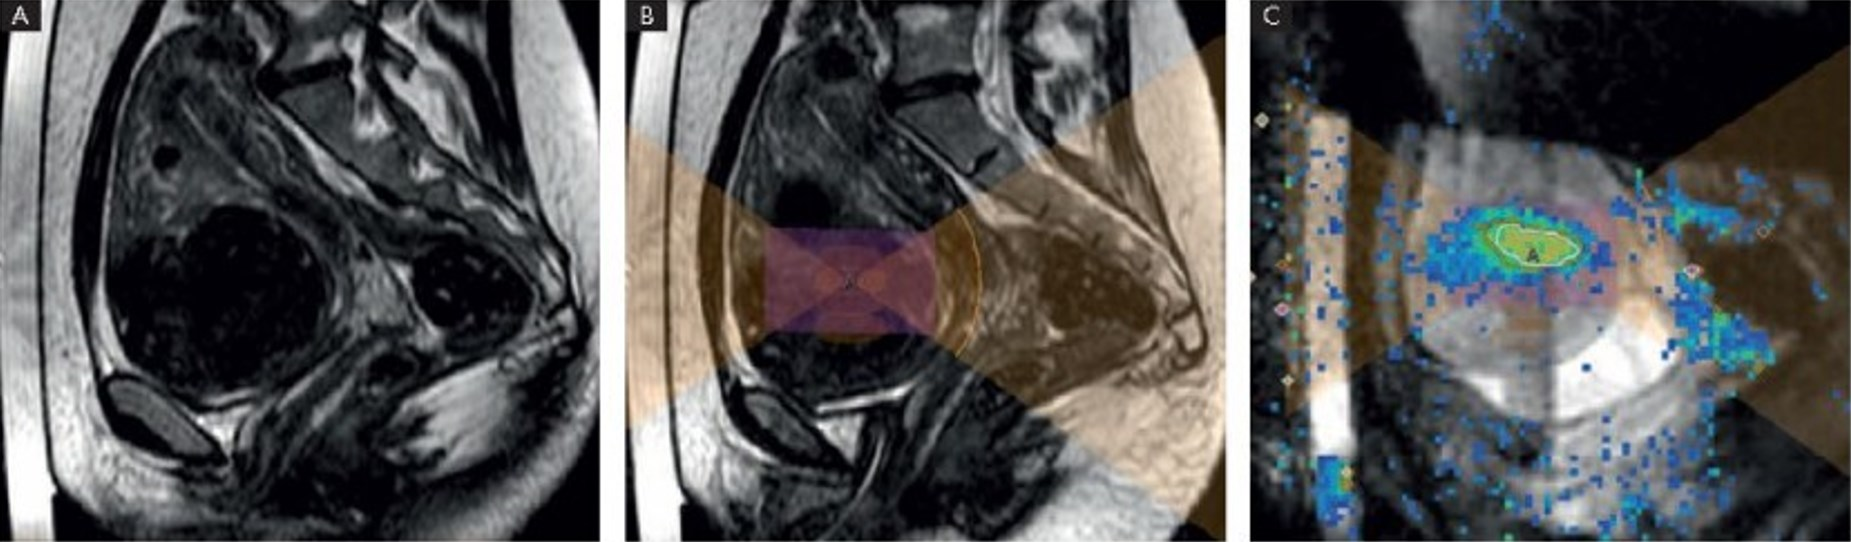
\includegraphics[width=\textwidth]{HIFU-example2}
    \caption{Real time temperature monitoring by MR-HIFU. The color indicates the chages in temperature. \cite{vanwijk2013}}
    \label{fig:HIFU_example}
\end{figure}

To solve this problem, computer simulation is introduced to help doctors estimate the temperature in bone tissue. Many methods have been developed to simulate HIFU system \cite{StochasticSim}. Most of them use ray tracing method, which treats the ultrasonic wave as ray beams propagating towards various medium. However, they are usually time consuming as they require the ray tracer to cast a large number of rays so that the sampled intensity can converge to the realistic values. In this report, a new ray tracer is proposed which keeps track of the divergence of the beam to estimate the intensity. The result shows that this new method can reduce the number of required ray and save some computational time.

\begin{figure}[h]
    \centering
    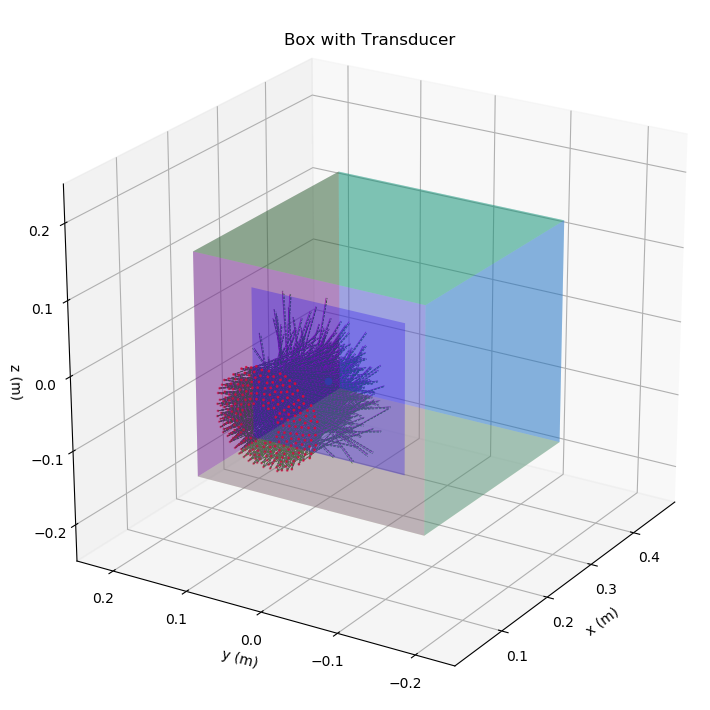
\includegraphics[width=0.5\textwidth]{box_transducer}
    \caption{Illustration of transducer elements casting ultrasound rays at a medium interface}
    \label{fig:transducer_coordinates}
\end{figure}

The study can be divided into the following steps:

\begin{itemize}
    \item Implement Trident-Ray tracing method
    \item Set up experiment where there's only one medium.
    \item Set up experiment where there're two fluid media.
    \item Run the simulation on the second experiment with various different parameters.
    \item compare the simulation result with old simulation method.
\end{itemize}

In the Method section, more detailed discussion about the theory and implementation will be presented. In the Result section, the output of the model in this study will be compared with the model of Modena et al \cite{Modena_2018}, based on similarity metrics.
